\documentclass[12pt]{article}
\usepackage[english]{babel}
\usepackage{amsmath, amssymb}
\usepackage{graphicx}
\usepackage{geometry}
\usepackage{hyperref}
\usepackage{fancyhdr}
\usepackage{float}
\usepackage{caption}

\geometry{margin=1in}
\pagestyle{fancy}
\fancyhf{}
\rhead{Set Covering Problem}
\lhead{Optimization Problem}
\rfoot{\thepage}

\title{Set Covering Problem\\\large PIA: Part IV}
\author{Operations Research, 032\\\large Team 6: Alan Alejandro Vargas González, 2086183}
\date{\ May, 2025}

\begin{document}

\maketitle

\section{Part IV: Final Results and Presentation}

\subsection{Final Data Execution}
To evaluate the scalability and robustness of the model, I tested with real-world set covering problems:

\begin{itemize}
    \item \texttt{rail2536.txt} (2536 rows, 1,081,841 columns)
    \item \texttt{rail4284.txt} (4284 rows, 1,092,610 columns)
    \item \texttt{rail4872.txt} (4872 rows, 968,672 columns)
\end{itemize}

\begin{table}[H]
\centering
\begin{tabular}{|l|c|c|c|c|}
\hline
\textbf{Instance} & \textbf{Selected Subsets} & \textbf{Cost} & \textbf{Time (s)} \\
\hline
\texttt{rail2536} & 80 & 13697.0 & 30.18 \\
\texttt{rail4284} & 128 & 5302.0 & 32.95 \\
\texttt{rail4872} & 91 & 27638.0 & 33.30 \\
\hline
\end{tabular}
\end{table}

\subsection{Result Visualization}

\begin{figure}[H]
    \centering
    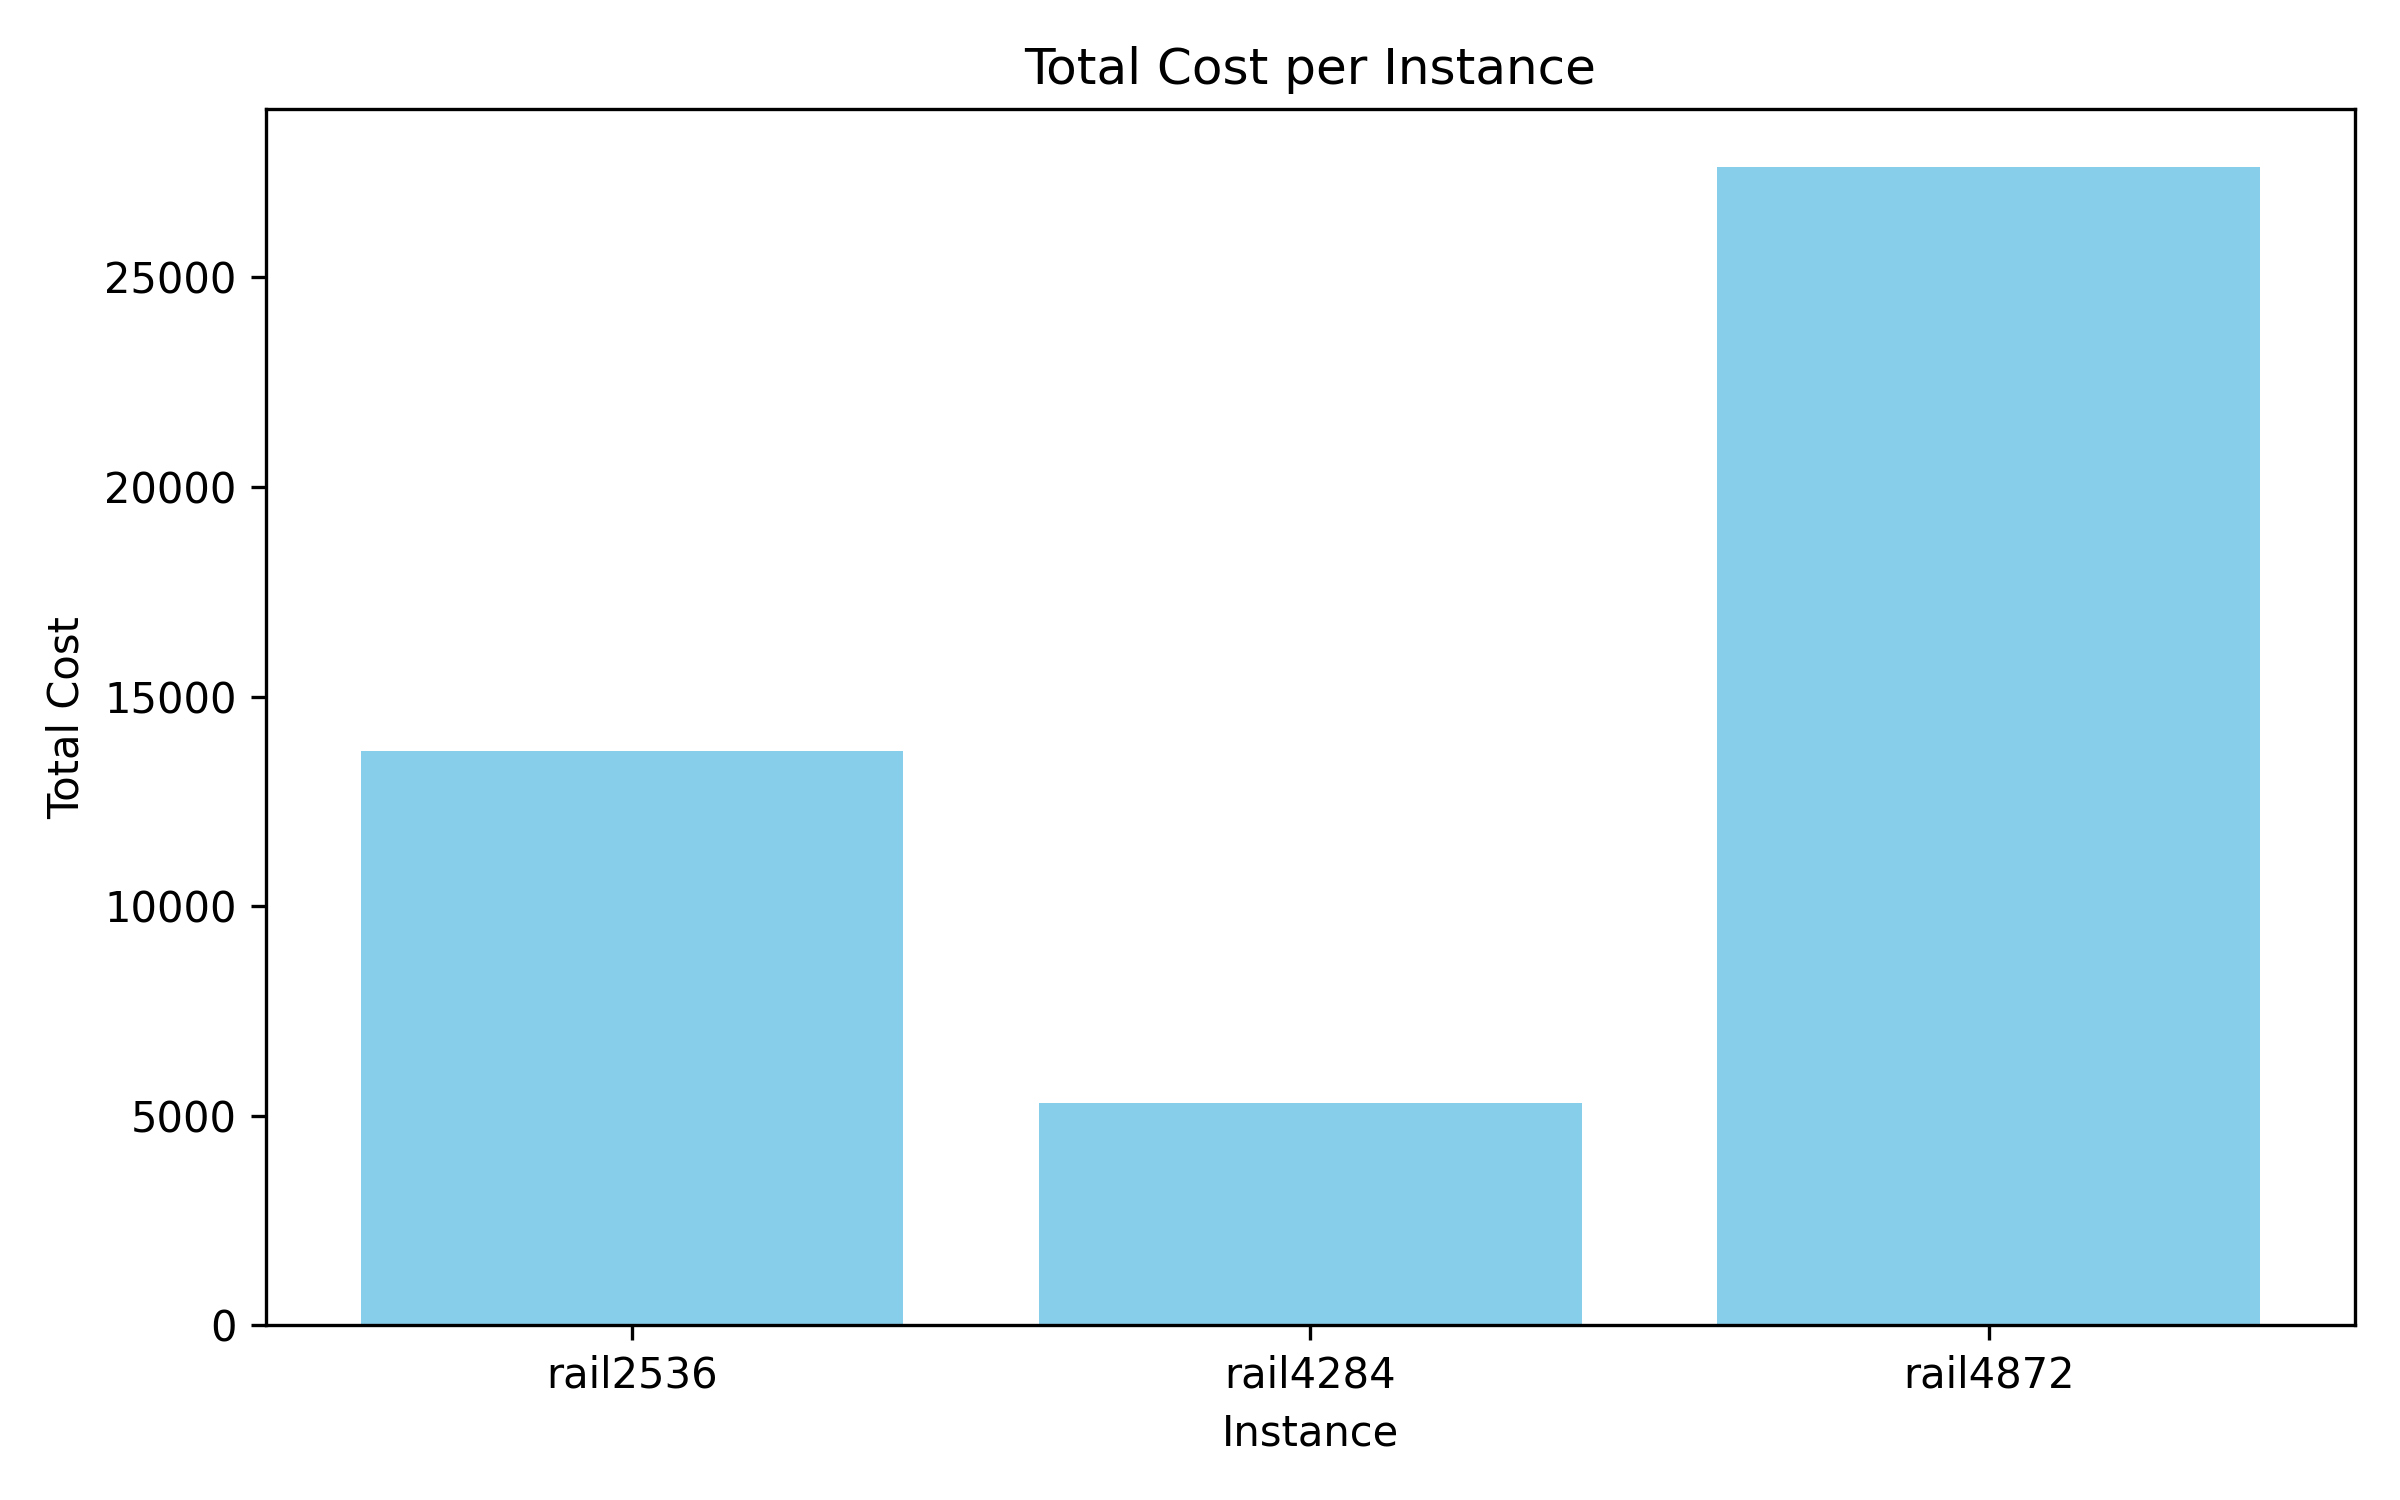
\includegraphics[width=0.75\textwidth]{instance_cost.png}
    \caption{Total cost per instance (railway dataset)}
\end{figure}

\begin{figure}[H]
    \centering
    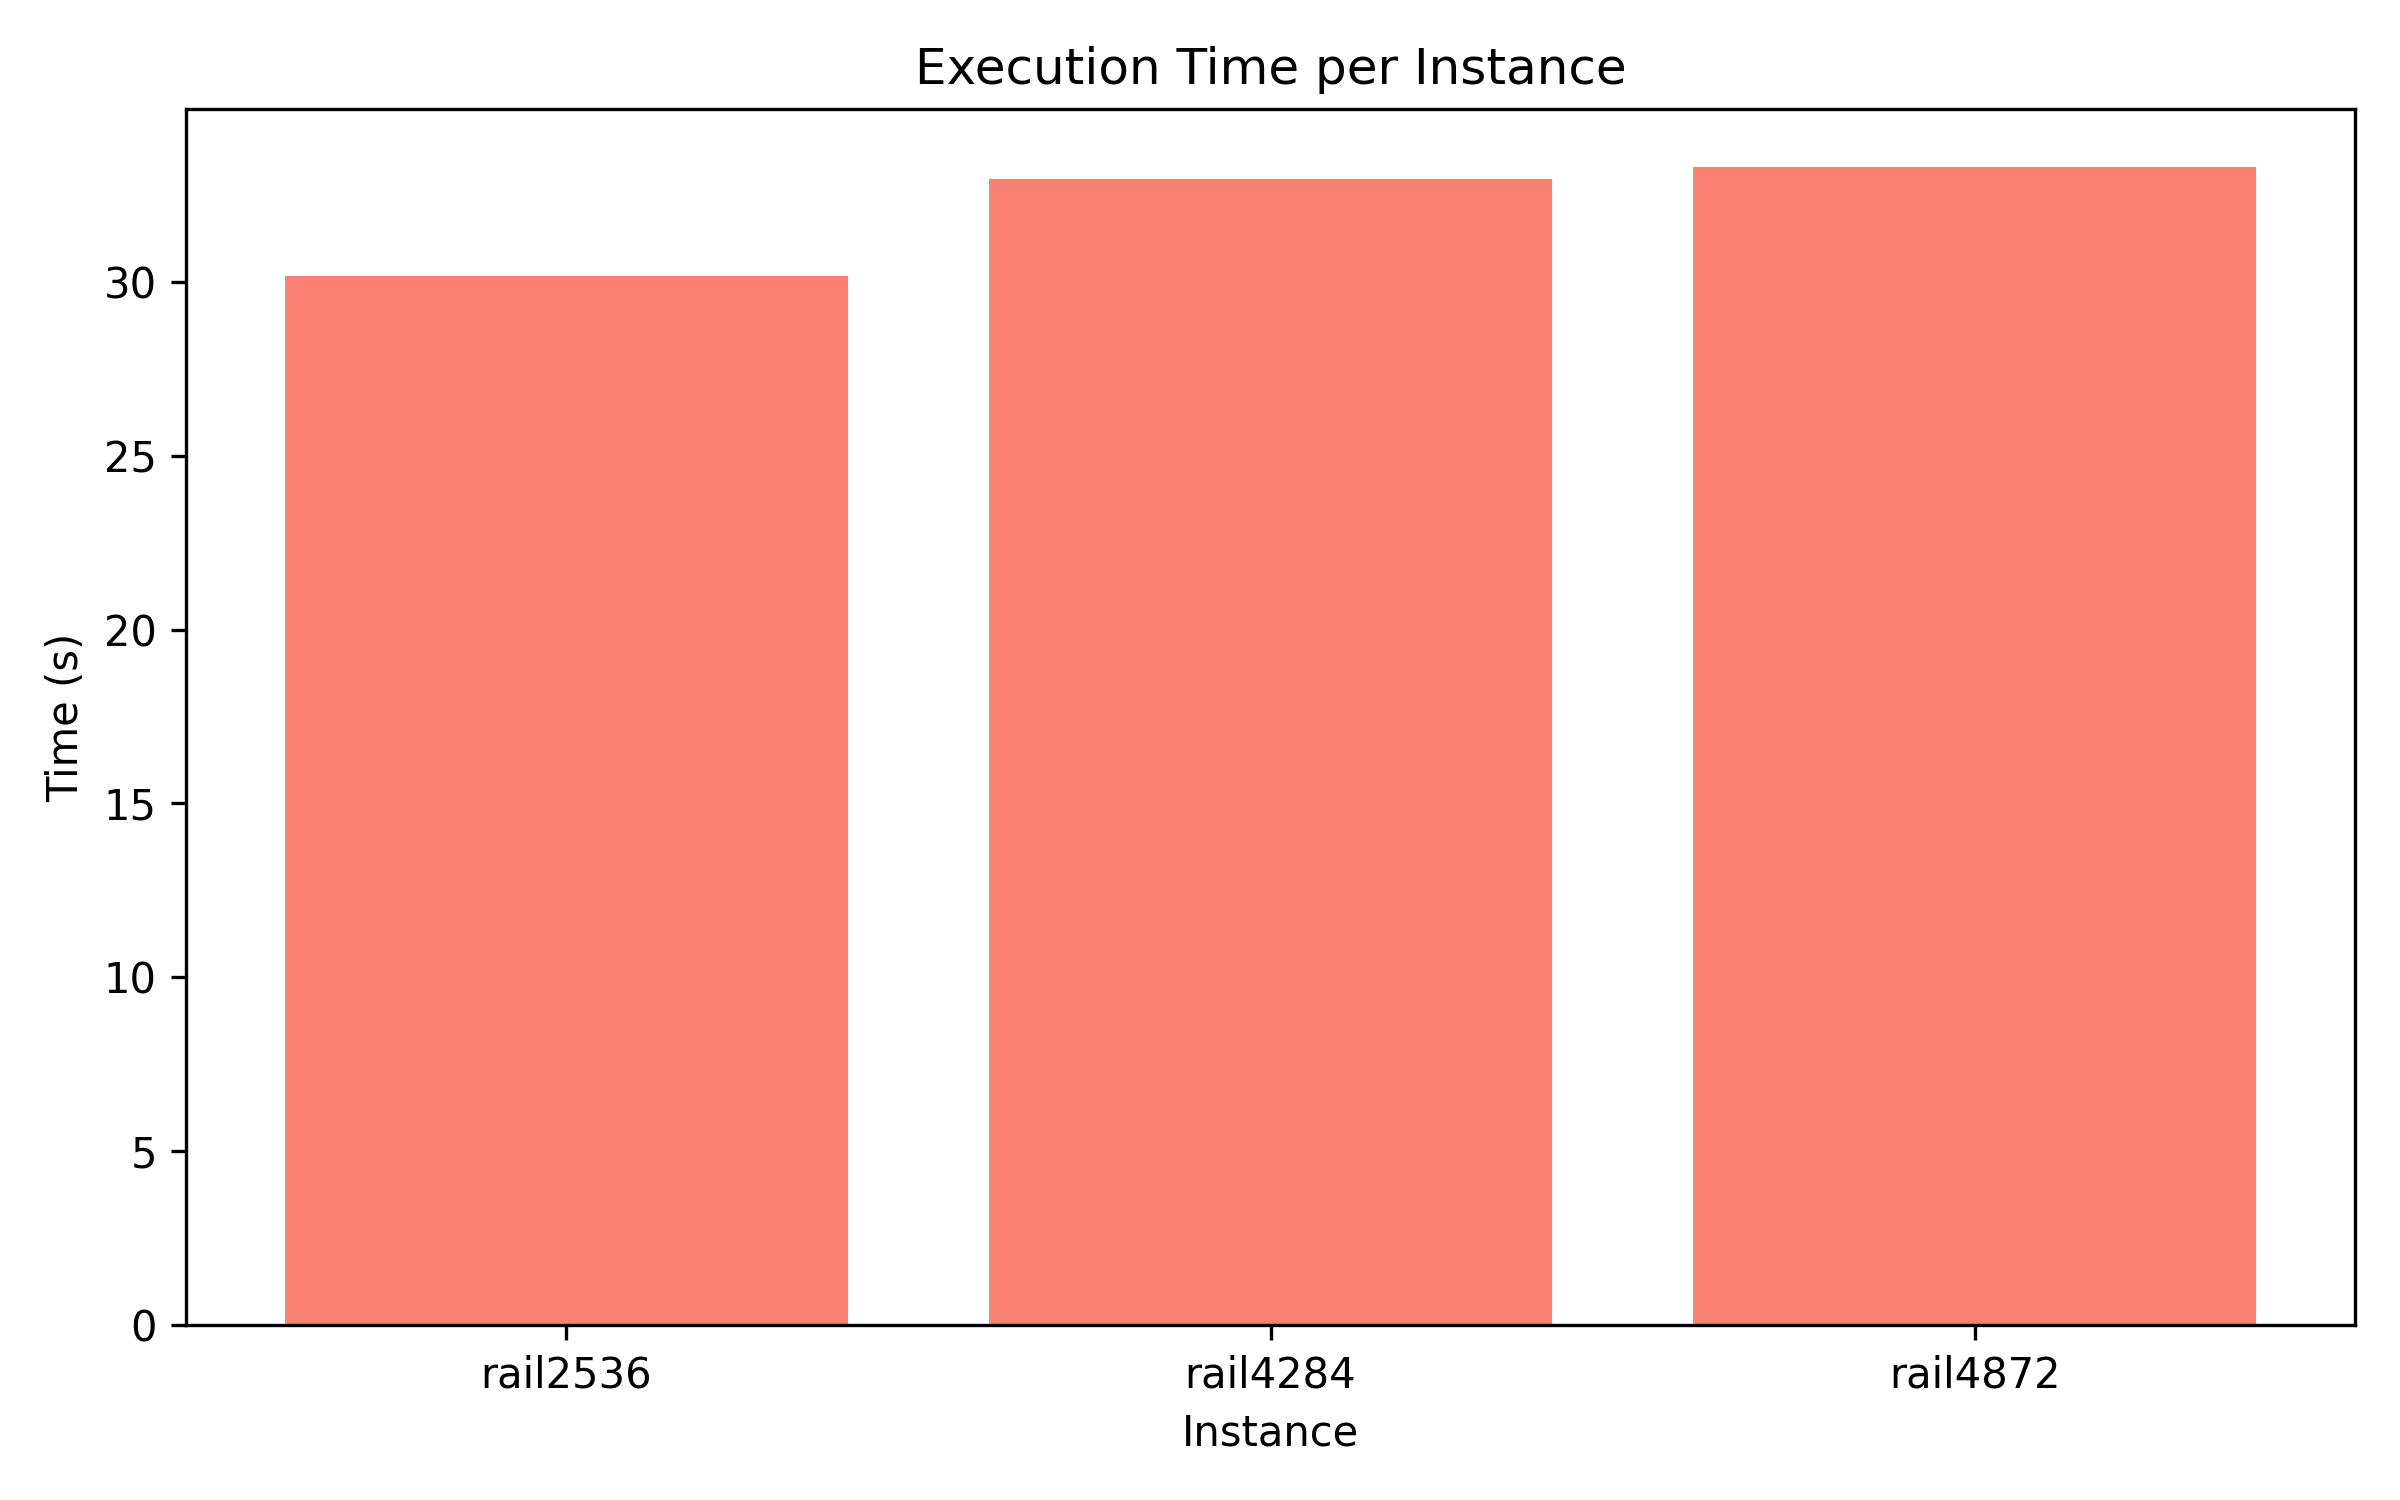
\includegraphics[width=0.75\textwidth]{instance_time.png}
    \caption{Execution time per instance (railway dataset)}
\end{figure}

\subsection{Result Interpretation}

\begin{itemize}
    \item \textbf{Scalability:} The solver remained stable and consistent in datasets with millions of variables.
    \item \textbf{Cost Variation:} Total cost varied significantly across datasets, highlighting structural differences in coverage density (e.g., some datasets may have cheap subsets capable of covering a broad set of elements).
    \item \textbf{Execution Time:} Execution time remained within 30-33 s, showing good performance given the large size of each dataset.
\end{itemize}

\subsection{Model Limitations and Assumptions}

\begin{itemize}
    \item Assumes deterministic and static input: no dynamic data.
    \item CBC solver was used; performance may vary with alternative solvers such as AMPL or Gurobi.
    \item No preprocessing was applied (e.g., eliminating redundant variables or rows), and no heuristic shortcuts were implemented.
\end{itemize}

\subsection{Deliverables}

\begin{itemize}
    \item \texttt{resultados.csv} with performance metrics
    \item \texttt{instance\_cost.png}, \texttt{instance\_time.png} with visual results
\end{itemize}

\end{document}
